\chapter{WAV Designer}
WAV designer is a single-cycle waveform generator optimized for the Elektron MD.\\
\\
WAV Designer is a 3 oscillator additive synthesis engine with a mixer.\\
\\
Each oscillator can be set to a unique waveform and pitch, the 3 oscillators are then mixed together and rendered in to a WAV file which can be transferred to the MD using the MIDI sample dump specification.\\
\\
To ensure the resulting waveform is played back optimally on the MD, WAV Designer performs all the heavy lifting for you. This involves calculating sample length, auto detecting loop points and setting a variable sample rate based on the fundamental frequency.

\section{Waveforms:}
\subsection{SIN:}Sine waveform with adjustable overtones (each overtone is an octave above the fundamental frequency)\\
\fbox{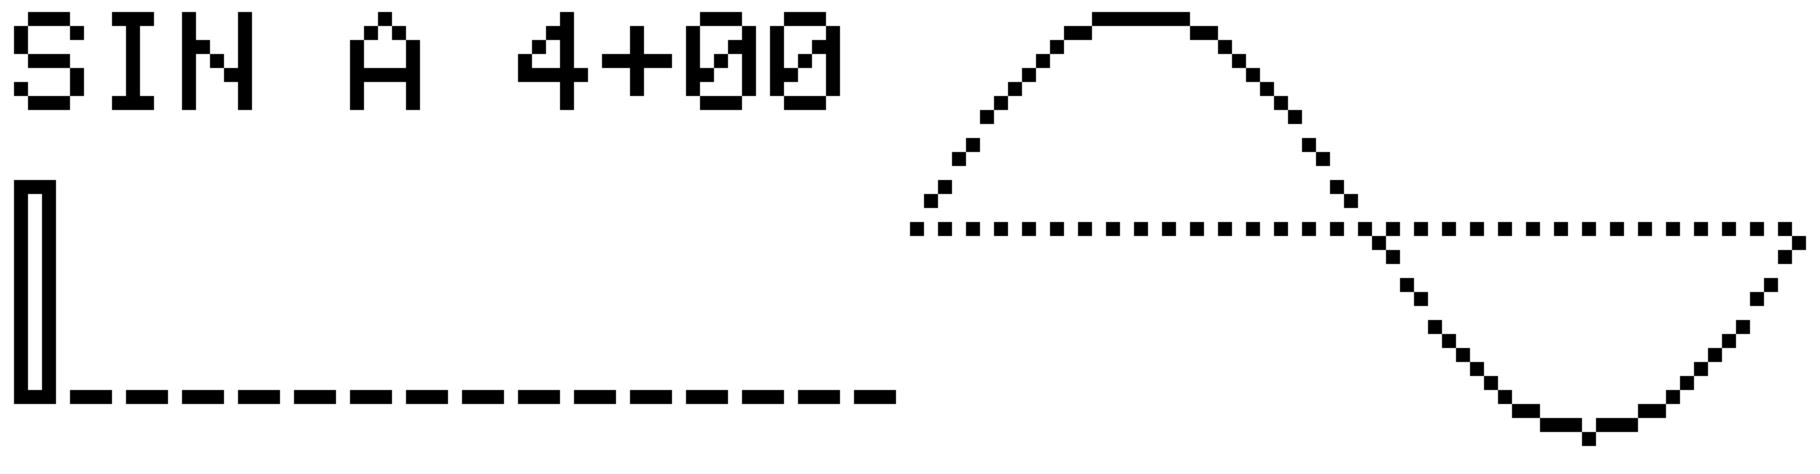
\includegraphics[scale=.40]{wav_designer_sine_init.png}}\\\\
\fbox{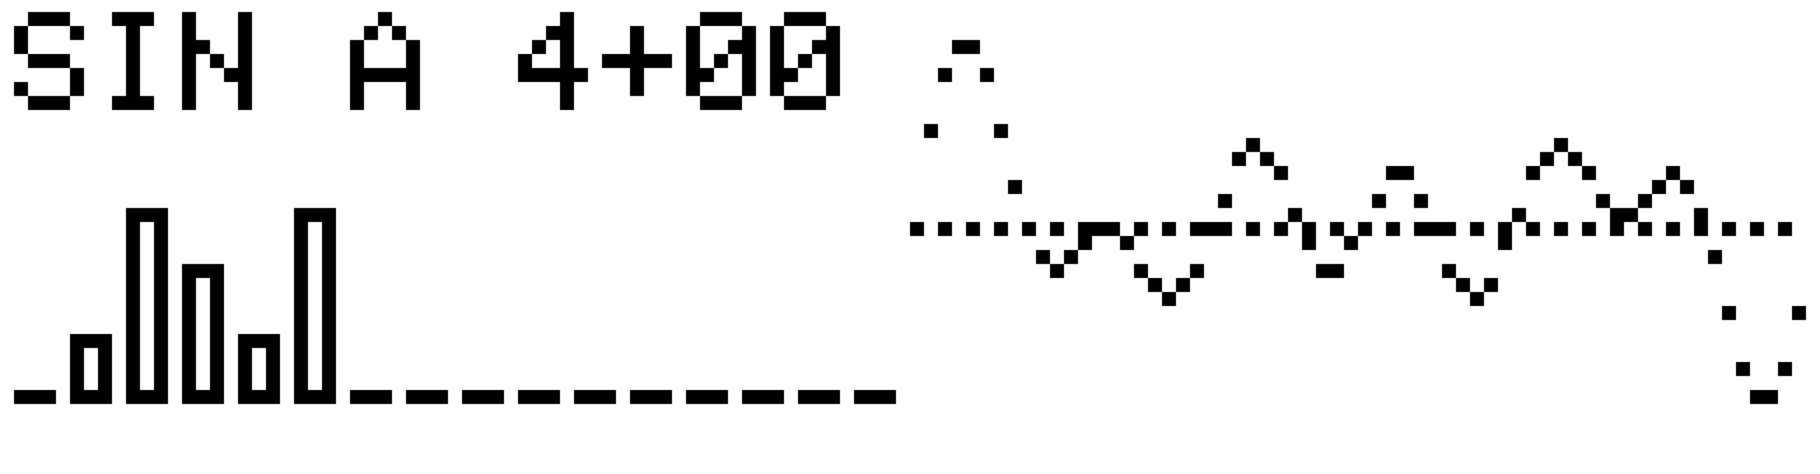
\includegraphics[scale=.40]{wav_designer_sin.png}}\\\\
\\Overtones are added by using the MD trigger interface and rotating \textbf{[Encoder 4]}.
\subsection{TRI:} Triangle waveform with adjustable width.\\
\fbox{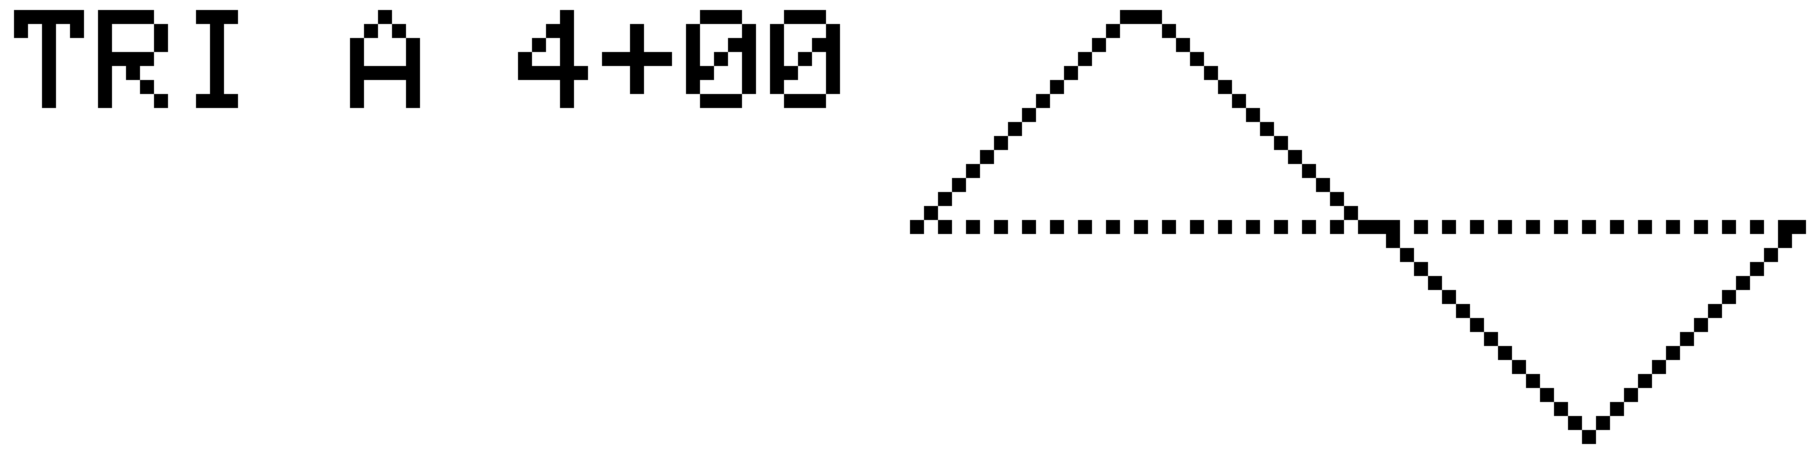
\includegraphics[scale=.40]{wav_designer_tri.png}}\\\\
\subsection{PUL:} Pulse/Square waveform with adjustable width.\\
\fbox{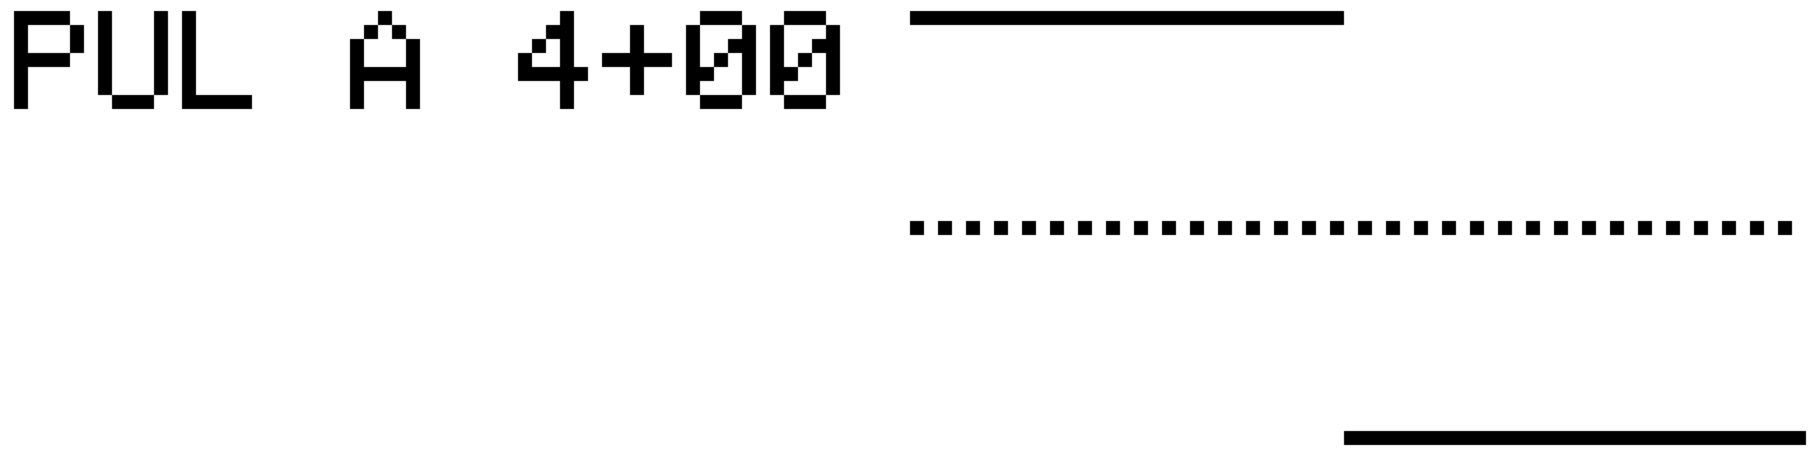
\includegraphics[scale=.40]{wav_designer_pulse.png}}\\\\
\subsection{SAW:}Sawthooth waveform with adjustable width\\
\fbox{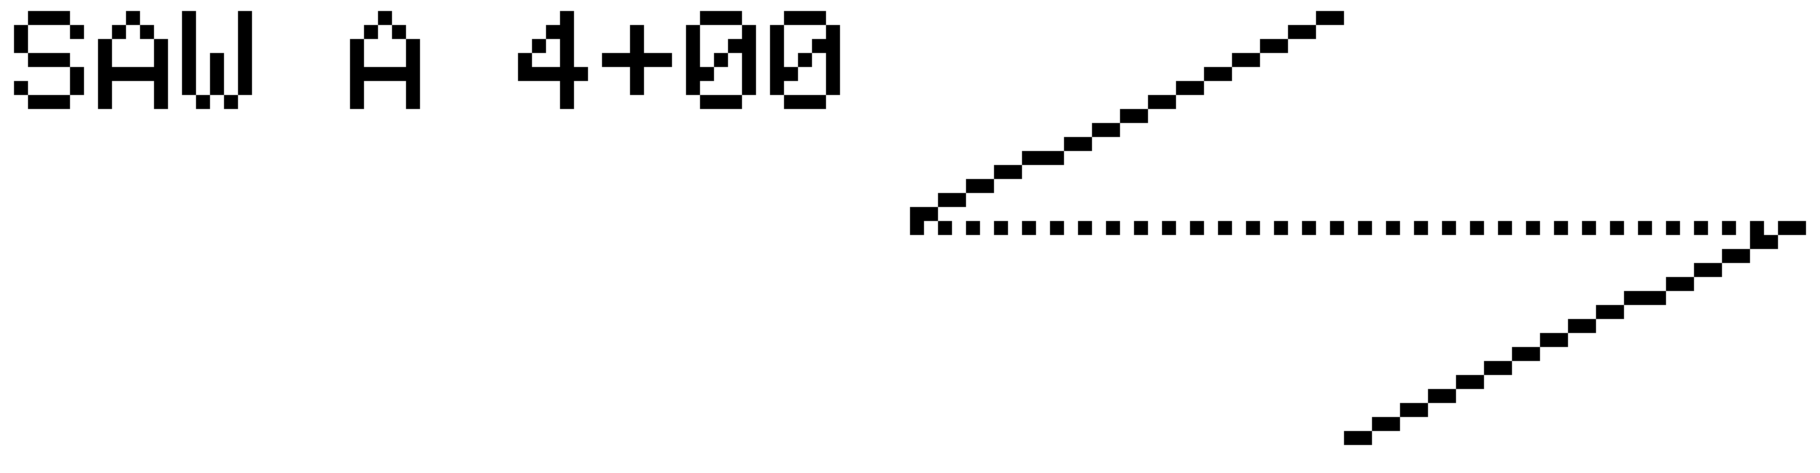
\includegraphics[scale=.40]{wav_designer_saw.png}}\\\\
\subsection{USR:}User defined waveform, 16 points with linear interpolation.\\
\fbox{
\includegraphics[scale=.40]{wav_designer_user.png}}\\\\
Sample values are modified by using the MD trigger interface and rotating \textbf{[Encoder 4]}.


\fbox{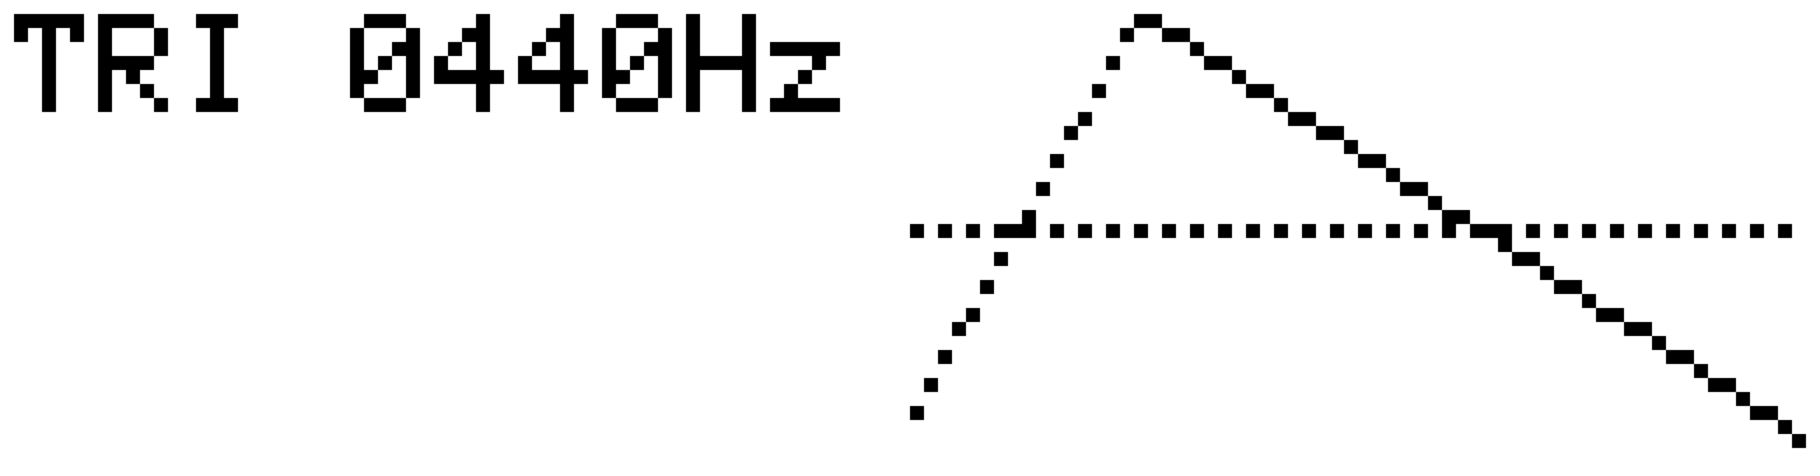
\includegraphics[scale=.40]{wav_designer_pulse_width.png}}\\\\


- 3 Oscillator Additive Synthesiser. Generates single cycle waveforms and sends
them to a MD sample slot.

\section{Wav Designer Pages:}
WAV designer is accessed through the PageSelect menu.

There are 4 pages to the WavDesigner. 
\textbf{[ Encoder 1-3]} buttons select oscillators 1-3 respectively.
\subsection{Oscillator Page}
- Oscillator wavform can be changed by pressing top left button repeteadly.

\subsection{Mixer Page:}
\fbox{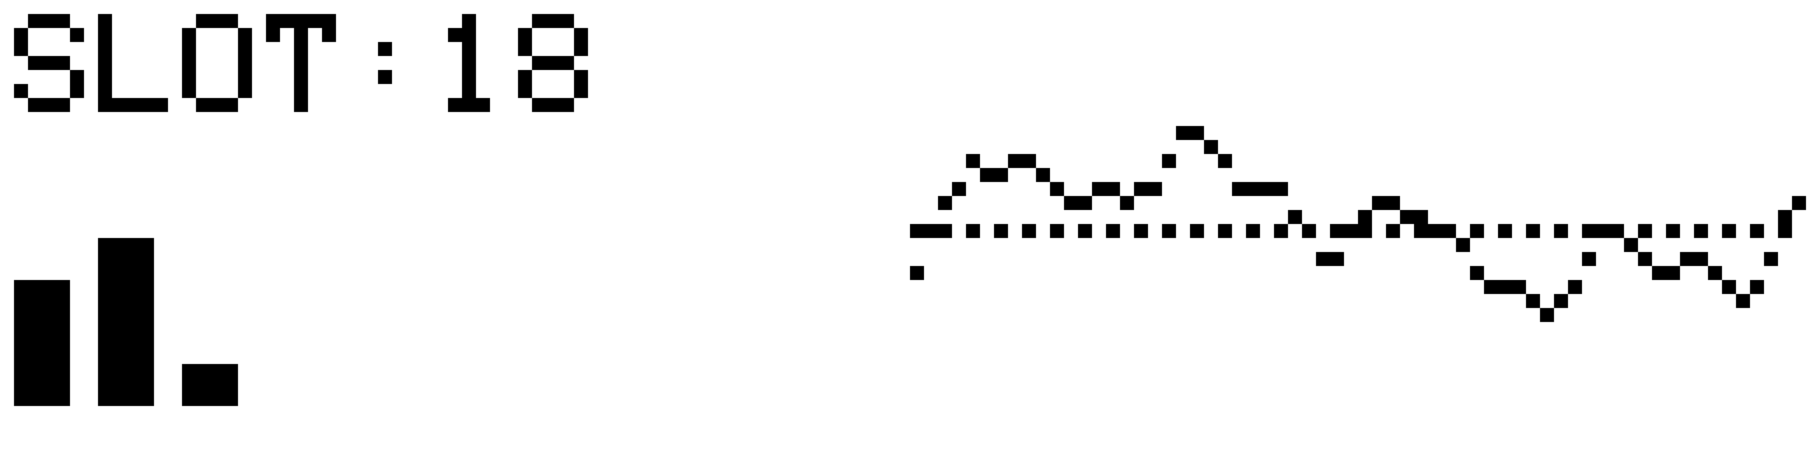
\includegraphics[scale=.40]{wav_designer_mixer.png}}\\\\




- The MD trigger interface together with encoder 4 can be used to
manipulate the SIN and USR waveforms.
- Encoder 1 pitch adjusts frequency by semitone.
- Encoder 2 is fine tune +-100 Cents
- Encoder 3 is pulse width.

Oscillator Mixer Page:
- The wav designer mixer page has volume levels for each of the oscillators.

- From the mixer page, top right button can be used to render and transmit the waveform.
(Some of the  MD GUI will lock up when receiving samples, see bug description
above)
- Encoders 1-3 adjust oscillator volume
- Encoder 4 adjusts MSD destination sample slot.

/subsection{Transferring Samples}
SAmples are transfrred from the Mixer Page. Once you are satisifed with the Mix, select a sample dump slot and press [Write] to transfer the sample. 

Alternatively, you can press the [Save] button to quickly load the Sample Manager page on the MD and select a receive position from the MD before transferring the sample.

\textbf{Important}: The MD firmware features a nasty bug that causes the user interface to stop responding if a sample dump is received at any point after specific SYSEX messages are requested. As MCL uses SYSEX for all communication with the MD, the MD's GUI will lock up after a sample is received from WavDesigner. The only known work around at this time is to reset the MD.